%!TEX root=../GaugeCNNTheory.tex


\subsection{میدان‌های بردار ویژگی مستقل از مختصات}
\label{sec:feature_fields}

فضاهای ویژگی شبکه‌های کانولوشنی مستقل از مختصات، فضاهای میدان‌های بردار ویژگی هستند.
مشابه مورد ضرایب بردارهای مماس، ضرایب عددی بردارهای ویژگی ملزم به تبدیل سازگار تحت تبدیل‌های گیج هستند.
قانون تبدیل خاص (نمایش گروهی) یک میدان ویژگی در اینجا نوع میدان آن را مشخص می‌کند – مثال‌های معمول شامل میدان‌های اسکالر، میدان‌های بردار مماس، میدان‌های تانسور عمومی، میدان‌های ویژگی منظم یا میدان‌های \lr{irrep} هستند.
بخش~\ref{sec:individual_fields} چنین میدان‌های ویژگی و قوانین تبدیل آن‌ها را معرفی می‌کند.
در بخش~\ref{sec:stacked_fields}، ما به طور مختصر فضاهای ویژگی مستقل از مختصات را تعریف می‌کنیم.
مشابه تعریف فضاهای ویژگی شبکه‌های کانولوشنی معمولی به عنوان انباشتی از چندین نقشه ویژگی، فضاهای ویژگی شبکه‌های کانولوشنی مستقل از مختصات شامل چندین میدان ویژگی مستقل هستند.




\subsubsection{میدان‌های بردار ویژگی منفرد}
\label{sec:individual_fields}
میدان‌های ویژگی کانولوشنی یک بردار ویژگی، که اطلاعات استنباط شده از یک همسایگی محلی از سیگنال ورودی را کدگذاری می‌کند، به هر نقطه از منیفولد تخصیص می‌دهند.
انباشت فضایی اطلاعات توسط یک کرنل کانولوشنی انجام می‌شود که میدان‌های ویژگی را در محیط خود \emph{نسبت به چارچوب مرجع محلی خود} \emph{اندازه‌گیری می‌کند}.
بنابراین ما گیج $\psi^A$ را فرض می‌کنیم که ترازهای کرنل را در یک همسایگی $U^A$ مشخص می‌کند.
نسبت به این گیج، کرنل یک میدان محلی هموار از پاسخ‌ها (مشاهدات) تولید خواهد کرد:
\begin{align}
	f^A:U^A\to\R^c \,,
\end{align}
که توسط یک بردار ویژگی عددی $c$-بعدی $f^A(p)$ در هر موقعیت $p\in U^A$ داده می‌شود.
فرض کنید یک میدان پاسخ دوم $f^B:U^B\to\R^c$ داده شده باشد که نسبت به گیج $\psi^B$ در $U^B$ استنباط شده است.
از آنجا که پاسخ یک کرنل به طور کلی به تراز آن بستگی دارد، انتظار می‌رود که $f^A$ و $f^B$ در همپوشانی $U^A\cap U^B$ مطابقت نداشته باشند.
بدون محدودیت‌های بیشتر، پاسخ‌های یک کرنل کانولوشن به طور دلخواه وابسته به گیج خواهند بود.

\begin{figure}
	\centering
	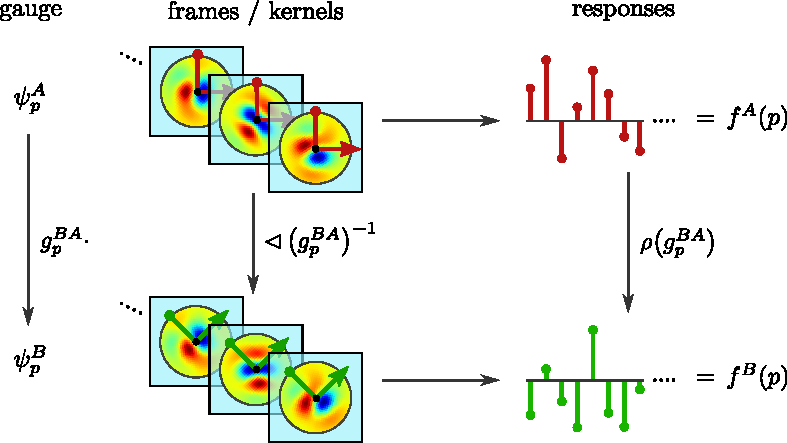
\includegraphics[width=.75\columnwidth]{figures/kernel_responses.pdf}
	\vspace*{1ex}
	\caption{\small
		پاسخ‌های عددی $f^A(p) \in\R^c$ و $f^B(p) \in\R^c$ کرنل‌هایی که بر اساس چارچوب‌های مختلف جهت‌گیری شده‌اند، به طور کلی منطبق نیستند.
		به منظور نمایش ضرایب عددی \emph{یکسان بردار ویژگی مستقل از مختصات} نسبت به گیج انتخاب شده، آن‌ها ملزم به ارتباط توسط تبدیل‌های گیج $\rho(g_p^{BA})$ هستند اگر گیج‌ها توسط~$g_p^{BA}$ مرتبط باشند.
		همانطور که در بخش~\ref{sec:gauge_CNNs_local} استخراج شده است، این الزام یک قید تناوب‌پذیری گیج را بر کرنل‌های کانولوشن تحمیل می‌کند.
	}
	\label{fig:gauge_trafos_feature_vector}
\end{figure}
		
		\begin{minipage}{\textwidth}
			\emph{اصل کوواریانس}، که توسط آلبرت انیشتین پیشنهاد شد \cite{Einstein1916German,Einstein1916English}، بیان می‌کند که:
			\vspace*{1.ex}
			\begin{center}
				\it
				«قوانین جهانشمول طبیعت باید توسط معادلاتی بیان شوند که برای همه سیستم‌های
				\\
				مختصات صادق باشند، یعنی نسبت به هر جایگزینی کوواریانت باشند.»
			\end{center}
			\vspace*{1.ex}
		\end{minipage}
		ما معتقدیم که اصل مشابهی باید در یادگیری عمیق هندسی نیز صادق باشد، یعنی استنتاج باید مستقل از هر دلخواهی در انتخاب چارچوب‌های مرجع باشد.
		با توجه به اینکه این دلخواهی در مختصات‌بندی‌ها دقیقاً توسط $G$-ساختار داده شده $\GM$ پوشش داده می‌شود، این امر به ویژه ایجاب می‌کند که \emph{ویژگی‌ها باید اشیاء هندسی مستقل از مختصات $\GM$ باشند}.%
		\footnote{
			در این نکته ما از \emph{کوواریانس عمومی} انیشتین منحرف می‌شویم، که همیشه تبدیل‌های گیج با مقدار $\GL{d}$ را در نظر می‌گیرد (متناظر با کوواریانس دیفئومورفیسم).
			تنظیم او در فرمول‌بندی ما برای $G=\GL{d}$ شامل شده است، با این حال، ما گروه ساختار فرضی را انعطاف‌پذیر نگه می‌داریم زیرا اکثر کاربردها گروه ساختار کاهش یافته را فرض خواهند کرد.
		}
		بنابراین ما کرنل‌های کانولوشن را طوری طراحی می‌کنیم که پاسخ‌های آن‌ها $f^A$ و $f^B$ میدان‌هایی از \emph{ضرایب بردار ویژگی} را کدگذاری کنند که \emph{یک میدان بردار ویژگی آزاد از مختصات $f$ را} به صورت محلی در گیج‌های مختلف نمایش می‌دهند.
		مجموعه‌ای از چنین میدان‌های ضریب عددی $f^X$، که نسبت به $G$-اطلس گیج‌های $\psi^X$ در همسایگی‌های $U^X$ که $M$ را پوشش می‌دهند بیان شده‌اند، معادل میدان ویژگی سراسری و آزاد از مختصات $f$ در~$M$ است.
		
		
		\begin{figure}
			\centering
			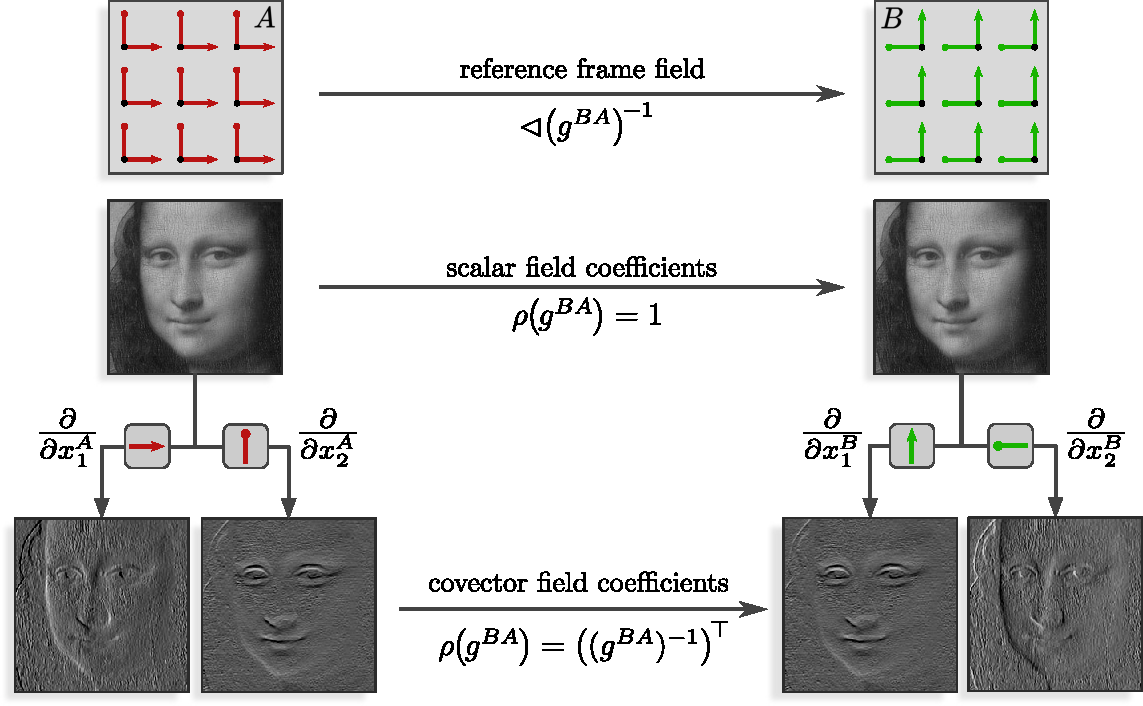
\includegraphics[width=.83\columnwidth]{figures/mona_lisa_gradient.pdf}
			\caption{\small
				مثال‌هایی از میدان‌های ضریب ویژگی در $M=\R^2$ از پردازش کلاسیک تصویر.
				\ \emph{بالا:}
				برای سادگی ما یک میدان چارچوب «موازی» فرض می‌کنیم و همان تبدیل گیج، چرخش به میزان $\pi/2$، را در هر نقطه $p\in M$ در نظر می‌گیریم.
				\ \emph{وسط:}
				مقادیر شدت یک تصویر خاکستری مستقل از انتخاب چارچوب‌های مرجع هستند.
				بنابراین آن‌ها توسط میدان‌های اسکالر مدل می‌شوند که با نمایش بدیهی $\rho(g)=1\ \forall g\in G$ مشخص می‌شوند.
				\ \emph{پایین:}
				دو کانال ضریب یک تصویر گرادیان از یک تصویر اسکالر با گرفتن مشتق‌ها در امتداد محورهای چارچوب محاسبه می‌شوند -- بنابراین آن‌ها وابسته به گیج هستند.
				تصاویر گرادیان نسبت به گیج‌های مختلف توسط نمایش گروهی $\rho(g)=(g^{-1})^\top$ مرتبط هستند و بنابراین به عنوان میدان‌های کوبردار (میدان‌های تانسور از نوع $(0,1)$ یا 1-فرم‌ها) شناسایی می‌شوند.
				برای چرخش نمایش داده شده به میزان $\pi/2$ این منجر به کانال اول جدید $(\nicefrac{\partial}{\partial x_1^B})$ معادل کانال دوم قدیمی $(\nicefrac{\partial}{\partial x_2^A})$ و کانال دوم جدید $(\nicefrac{\partial}{\partial x_2^B})$ معادل منفی کانال اول قدیمی $(\nicefrac{\partial}{\partial x_1^A})$ می‌شود.
				نسبت به چارچوب‌های مرجع مربوطه، هر دو میدان ضریب یکسان میدان گرادیان (آزاد از مختصات) را کدگذاری می‌کنند.
				بنابراین توصیف به طور خودکار مستقل از مختصات است.
			}
			\label{fig:feature_field_gradient}
		\end{figure}
				
				برای اینکه این میدان ویژگی آزاد از مختصات به خوبی تعریف شود، یعنی مستقل از مختصات $\GM$ باشد، میدان‌های ضریب محلی (یا پاسخ‌های کرنل) ملزم به دوخته شدن سازگار از طریق نگاشت‌های گذار با مقدار $G$ هستند.
				بنابراین آن‌ها باید به روشی اصولی تحت تبدیل‌های گیج تبدیل شوند.
				از آنجا که ما با فضاهای بردار ویژگی سر و کار داریم، این تبدیل‌ها معمولاً خطی در نظر گرفته می‌شوند، یعنی آن‌ها توسط \emph{نمایش‌های گروهی} خطی مدل می‌شوند:
				\begin{align}\label{eq:group_representation}
					\rho:G\to\GL{c}
				\end{align}
				از گروه ساختار $G\leq\GL{c}$، که بر $\R^c$ عمل می‌کند و شرط $\rho(gh)=\rho(g)\rho(h)\ \forall\ g,h\in G$ را برآورده می‌کند.%
				\footnote{\label{footnote:repr_group_homomorphism}
					این شرط تضمین می‌کند که نمایش‌ها همومورفیسم‌های گروهی هستند، یعنی نگاشت‌هایی که ساختار گروهی~$G$ را رعایت می‌کنند.
					بنابراین عمل‌های گروه ساختار بر فضای مماس و فضاهای ضریب بردار ویژگی سازگار هستند.
				}
				مشابه تبدیل ضرایب بردار مماس در معادله~\eqref{eq:components_leftaction}، ضرایب بردار ویژگی سپس تعریف می‌شوند که تحت یک تبدیل گیج با مقدار $G$ مانند $g_p^{BA}=\psi_p^B\!\circ\!\left(\psi_p^A\right)^{-1}$ تبدیل شوند:
				\begin{align}\label{eq:gauge_trafo_features}
					f^B(p)\ :=\ \rho\big( g_p^{BA}\big) f^A(p) \,,
				\end{align}
				که در آن $p\in U^A\cap U^B$؛ برای بصری‌سازی به شکل~\ref{fig:gauge_trafos_feature_vector} مراجعه کنید.
				با ساخته شدن برای تبدیل همگام، فضاهای چارچوب‌های مرجع، ضرایب بردار مماس و ضرایب بردار ویژگی گفته می‌شود که با یکدیگر $G$-\emph{مرتبط} هستند.
				توجه داشته باشید که ساخت از طریق یک $G$-نمایش $\rho$ به طور کلی تبدیل‌های گیج با مقدار $\GL{d}$ را توصیف \emph{نمی‌کند}، یعنی ویژگی‌های کاملاً مستقل از مختصات.
				بنابراین بردارهای ویژگی استخراج شده تنها بیان به خوبی تعریف شده‌ای نسبت به چارچوب‌ها در $G$-ساختار در نظر گرفته شده $\GM$ خواهند داشت، که توسط اصطلاح «استقلال از مختصات $\GM$» پوشش داده می‌شود.
				
				
				انتخاب‌های مختلف نمایش‌ها $\rho_i$ \emph{انواع} مختلفی از میدان‌های ویژگی را تولید می‌کنند همانطور که در شکل~\ref{fig:feature_field_gradient} نمونه‌سازی شده است.
				به عنوان مثال، نمایش بدیهی، $\rho(g)=1\ \forall g\in G$، رفتار تبدیل \emph{میدان‌های اسکالر} $s^A(p)\ \mapsto\ s^B(p)\ :=\ 1\cdot s^A(p)$ را توصیف می‌کند، که ضرایب عددی آن‌ها تحت تبدیل‌های گیج ناوردا هستند.
				مثال‌هایی از میدان‌های اسکالر شامل تصاویر خاکستری، میدان‌های دما، میدان‌های فشار یا توزیع‌های احتمال در $M$ هستند.
				ضرایب \emph{میدان‌های بردار مماس} مانند $v^A(p)\ \mapsto\ v^B(p)\ :=\ g_p^{BA}v^A(p)$ تبدیل می‌شوند و بنابراین با نمایش گروهی $\rho(g)=g$ مطابقت دارند.
				مثال‌هایی برای میدان‌های بردار شامل جریان نوری یا میدان‌های سرعت باد هستند.
				میدان‌های تانسور عمومی‌تر از نوع $(r,s)$ توسط نمایش‌های حاصل‌ضرب تانسوری $\rho(g) = \otimes^s\left(g^{-1}\right)^{\!\top} \otimes^r g$ توصیف می‌شوند.
				آن‌ها به عنوان مثال تصاویر تانسور انتشار، تانسورهای میدان الکترومغناطیسی یا تانسورهای تنش را مدل می‌کنند.
				انتخاب رایج برای گروه‌های ساختار گسسته \emph{نمایش‌های منظم} هستند که مجموعه محدود عملیات گروهی را توسط ماتریس‌های جایگشت تحقق می‌بخشند.
				نمایش‌های منظم به عنوان تقارن‌های دقیق شبکه‌های کریستالی، شبکه‌های اسپین یا شبکه‌های پیکسل ظاهر می‌شوند~\cite{Cohen2016-GCNN,Hoogeboom2018-HEX,winkels3DGCNNsPulmonary2018,Worrall2018-CUBENET,gaugeIco2019}.
				علاوه بر این، آن‌ها معمولاً به عنوان تقریب گسسته گروه‌های ساختار پیوسته استفاده می‌شوند، به عنوان مثال گروه‌های چرخشی $C_N\leq\SO{2}$ برای تقریب چرخش‌های پیوسته~\cite{Weiler2018SFCNN,bekkers2018roto,Weiler2019_E2CNN,bekkers2020bspline,Marcos2017-VFN}.
				آن‌ها از اهمیت عملی زیادی برخوردارند زیرا تبدیل ویژگی‌های شبکه‌های کانولوشنی گروهی را توصیف می‌کنند~\cite{Cohen2016-GCNN}.
				میدان‌های ویژگی که تحت \emph{نمایش‌های کاهش‌ناپذیر} (\lr{irrep}) تبدیل می‌شوند در~\cite{Worrall2017-HNET,3d_steerableCNNs,Thomas2018-TFN,Kondor2018-NBN,anderson2019cormorant,Weiler2019_E2CNN,jiang2019spherical} بررسی شدند.%
				\footnote{
					\label{footnote:feature_field_irrep_decomposition}
					توسط قضیه \lr{Peter-Weyl}، هر نمایش یکانی از یک گروه فشرده می‌تواند از طریق تغییر پایه به مجموع مستقیم \lr{irreps} تجزیه شود.
					این دلالت دارد بر اینکه هر عملیات شبکه عصبی \emph{خطی} بین نمایش‌های عمومی می‌تواند (پس از تغییر پایه) بر حسب عملیات بین \lr{irreps} درک شود~\cite{Weiler2019_E2CNN,lang2020WignerEckart}.
					در مقابل، انتخاب خاص نمایش، یعنی تغییر پایه نسبت به \lr{irreps} موجود در آن، برای هر لایه شبکه \emph{غیرخطی} \emph{اهمیت دارد}.
				}
				مروری دقیق‌تر و معیاری گسترده از انواع میدان یا نمایش‌های مختلف در یادگیری عمیق در~\cite{Weiler2019_E2CNN} ارائه شد.
				
				
				برای کامل بودن می‌خواهیم اشاره کنیم که میدان‌های بردار ویژگی آزاد از مختصات به طور رسمی به عنوان برش‌های هموار $f\in\Gamma(\A)$ از یک \emph{بندل بردار ویژگی} $\A\piAarrow M$ تعریف می‌شوند که با $G$-ساختار $\GM$ مرتبط است و فضاهای ضریب بردار ویژگی $\R^c$ را به عنوان فیبرهای معمول دارد.
				بردارهای ضریب $f^A(p)$ و $f^B(p)$ در $\R^c$ تسهیمات محلی از یک بردار ویژگی آزاد از مختصات $f(p) \in \A_p \cong \R^c$ هستند، و مشابه ضرایب $v^A=\psi_p^A(v)$ و $v^B=\psi_p^B(v)$ از یک بردار مماس $v\in \TpM$ تعریف می‌شوند.
				توجه داشته باشید که، در حالی که هم‌ریخت هستند، فضاهای ویژگی $\A_p \cong \A_q$ در نقاط مختلف $p\neq q$ از~$M$ از یکدیگر متمایز هستند، به طوری که عناصر آن‌ها نمی‌توانند با هم جمع شوند.
				انتقال‌دهنده‌های موازی، که در بخش‌های~\ref{sec:transport_local} و~\ref{sec:bundle_transport} مورد بحث قرار گرفته‌اند، هم‌ریختی‌هایی بین فضاهای بردار ویژگی مختلف فراهم می‌کنند، که امکان جمع ویژگی‌ها را (پس از انتقال آن‌ها به همان فضای برداری) فراهم می‌کند.
				از آنجا که این تعاریف کاملاً فنی هستند، ما جزئیات آن‌ها را فعلاً رد می‌کنیم و خواننده علاقه‌مند را به بخش~\ref{sec:G_associated_bundles} ارجاع می‌دهیم.
				
				
				
				
				
				
				
				
\subsubsection{میدان‌های ویژگی انباشته و فضاهای ویژگی مستقل از مختصات}
\label{sec:stacked_fields}

\begin{wrapfigure}[12]{r}{0.365\textwidth}
	\vspace*{-4.25ex}
	\hfill
	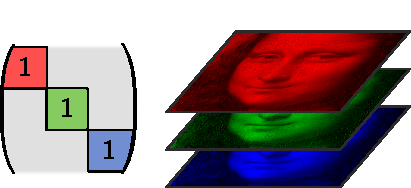
\includegraphics[width=.95\linewidth]{figures/feature_field_RGB.pdf}%
	\vspace*{.0ex}
	\captionsetup{width=.35\textwidth}
	\caption{\small
						سه کانال رنگ یک تصویر \lr{RGB} به عنوان میدان‌های اسکالر شناسایی می‌شوند، بنابراین فضای ویژگی کامل طبق $\rho(g) = (\mkern1.5mu 1 \mkern1.5mu) \oplus (\mkern1.5mu 1 \mkern1.5mu) \oplus (\mkern1.5mu 1 \mkern1.5mu)$ تبدیل می‌شود.
					}
					\label{fig:feature_space_RGB}
				\end{wrapfigure}%
				فضاهای ویژگی شبکه‌های کانولوشنی معمولی شامل چندین نقشه ویژگی هستند.
				به طور مشابه، ما فضاهای ویژگی شبکه‌های کانولوشنی مستقل از مختصات را تعریف می‌کنیم که شامل چندین میدان ویژگی $f_i$ از انواع بالقوه متفاوت $\rho_i$ و ابعاد $c_i$ باشند.
				بنابراین یک میدان کامل از فعالسازی‌های یک فضای ویژگی از یک شبکه کانولوشنی مستقل از مختصات به عنوان \emph{مجموع مستقیم} تعریف می‌شود%
				\footnote{
					مجموع مستقیم $\oplus$ بردارهای $f_i(p)$ را می‌توان به عنوان «انباشت» آن‌ها در یک بردار پیوسته در نظر گرفت.
					به طور سازگار با این، مجموع مستقیم نمایش‌های $\rho_i$ را می‌توان به عنوان ساخت یک ماتریس قطری بلوکی حاوی $\rho_i$ به عنوان بلوک‌ها در نظر گرفت؛ به اشکال~\ref{fig:feature_space_RGB} و~\ref{fig:feature_spaces_oplus} مراجعه کنید.
				}
				\begin{align}\label{eq:feature_field_full}
					f = \scalebox{1.1}{$\bigoplus$}_i f_i
				\end{align}
				از میدان‌های منفرد.
				هر نقشه ویژگی از یک شبکه کانولوشنی معمولی موقعیت یک ویژگی خاص را کدگذاری می‌کند و به طور مستقل تبدیل می‌شود هنگامی که ورودی شبکه جابجا می‌شود.
				میدان‌های ویژگی منفرد $f_i$ شبکه‌های کانولوشنی مستقل از مختصات $\GM$ هم موقعیت و هم $G$-پوز یک ویژگی را کدگذاری می‌کنند.
				در مقابل نقشه‌های ویژگی معمولی، میدان‌های ضریب آن‌ها، به عنوان مثال $f_i^A$، علاوه بر این تضمین شده‌اند که به طور مستقل از یکدیگر تحت تبدیل‌های گیج همانطور که توسط نوع آن‌ها ${\rho_i:G\to\GL{{c_i}}}$ مشخص شده است، تبدیل شوند.
				یک نمایش عددی محلی $f^A = \bigoplus_i f_i^A$ از میدان ویژگی کامل در معادله~\eqref{eq:feature_field_full} بنابراین طبق مجموع مستقیم نمایش‌های منفرد تبدیل می‌شود، یعنی:
				\begin{align}
					\rho = \scalebox{1.1}{$\bigoplus$}_i \rho_i \,.
				\end{align}
				تبدیل مستقل میدان‌های منفرد تحت $\rho$، که در شکل~\ref{fig:feature_spaces_oplus} بصری‌سازی شده است، از ساخت روشن است:
				\begin{align}
					\rho(g)f^A
					\,=\, \left(\scalebox{1.1}{$\bigoplus$}_i \rho_i(g)\right) \! \left(\scalebox{1.1}{$\bigoplus$}_i f_i^A\right)
					\,=\, \scalebox{1.1}{$\bigoplus$}_i \! \left(\rho_i(g) f_i^A\right)
				\end{align}
				
				\begin{figure}
					\centering
					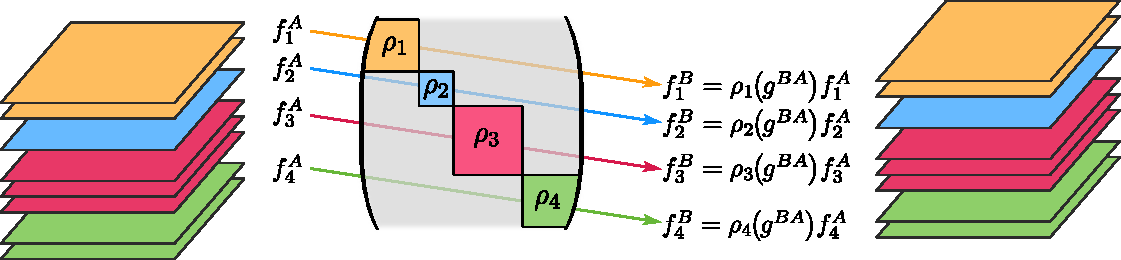
\includegraphics[width=.94\textwidth]{figures/feature_field_repr_examples.pdf}
					\vspace*{0ex}
					\caption{\small
						یک فضای ویژگی کامل شامل چندین میدان ویژگی منفرد $f_i$ از انواع بالقوه متفاوت $\rho_i$ و ابعاد $c_i$ است.
						از طریق گیج $\psi^A$، به صورت محلی توسط میدان‌های ضریب $f_i^A: U^A \to \R^{c_i}$ نمایش داده می‌شود.
						میدان‌های ضریب در گیج دیگر $\psi_B$ از طریق تبدیل گیج $f_i^B = \rho_i\big(g^{BA}\big)f_i^A$ مرتبط هستند.
						ضرایب هر میدان منفرد به طور مستقل تبدیل می‌شوند، بنابراین نمایش مدل‌سازی کل فضای ویژگی توسط مجموع مستقیم داده می‌شود، در اینجا $\bigoplus_i \!\rho_i = \rho_1 \oplus \rho_2 \oplus \rho_3 \oplus \rho_4$.
					}
					\label{fig:feature_spaces_oplus}
					\end{figure}

						به عنوان یک مثال عملی از فضای ویژگی مستقل از مختصات متشکل از چندین میدان، تصویر \lr{RGB} را همانطور که در شکل~\ref{fig:feature_space_RGB} نشان داده شده است، در نظر بگیرید.
						مانند تصویر خاکستری در شکل~\ref{fig:feature_field_gradient}، کانال‌های رنگ منفرد مقادیر شدت را کدگذاری می‌کنند که تحت تبدیل‌های گیج ناوردا هستند.
						بنابراین تصویر \lr{RGB} کامل باید با سه میدان اسکالر شناسایی شود که هر کدام به طور مستقل تحت نمایش بدیهی «تبدیل» می‌شوند.
						همه میدان‌های ویژگی منفرد نیازی نیست که از همان نوع $\rho_i$ باشند.
						به عنوان مثال، در یک کاربرد پیش‌بینی آب و هوا، سیگنال ورودی ممکن است شامل میدان‌های اسکالر کدگذاری کننده ویژگی‌هایی مانند دما یا فشار و میدان‌های برداری مانند سرعت‌های باد باشد.
						توصیف به عنوان میدان‌های $\rho_i$ از انواع مربوطه، پردازش هندسی صحیح چنین داده‌هایی را تضمین می‌کند.
						در حالی که انواع میدان $\rho_i$ ورودی و خروجی یک شبکه معمولاً توسط وظیفه یادگیری داده می‌شوند، انواع میدان استفاده شده در لایه‌های مخفی توسط کاربر به عنوان یک فراپارامتر مشابه انتخاب کانال‌ها برای یک شبکه کانولوشنی معمولی انتخاب می‌شوند.